
\chapter{Background and Related Work}
\label{chapter:Related_Work}

%\begin{figure}[h]
  %\centering
    %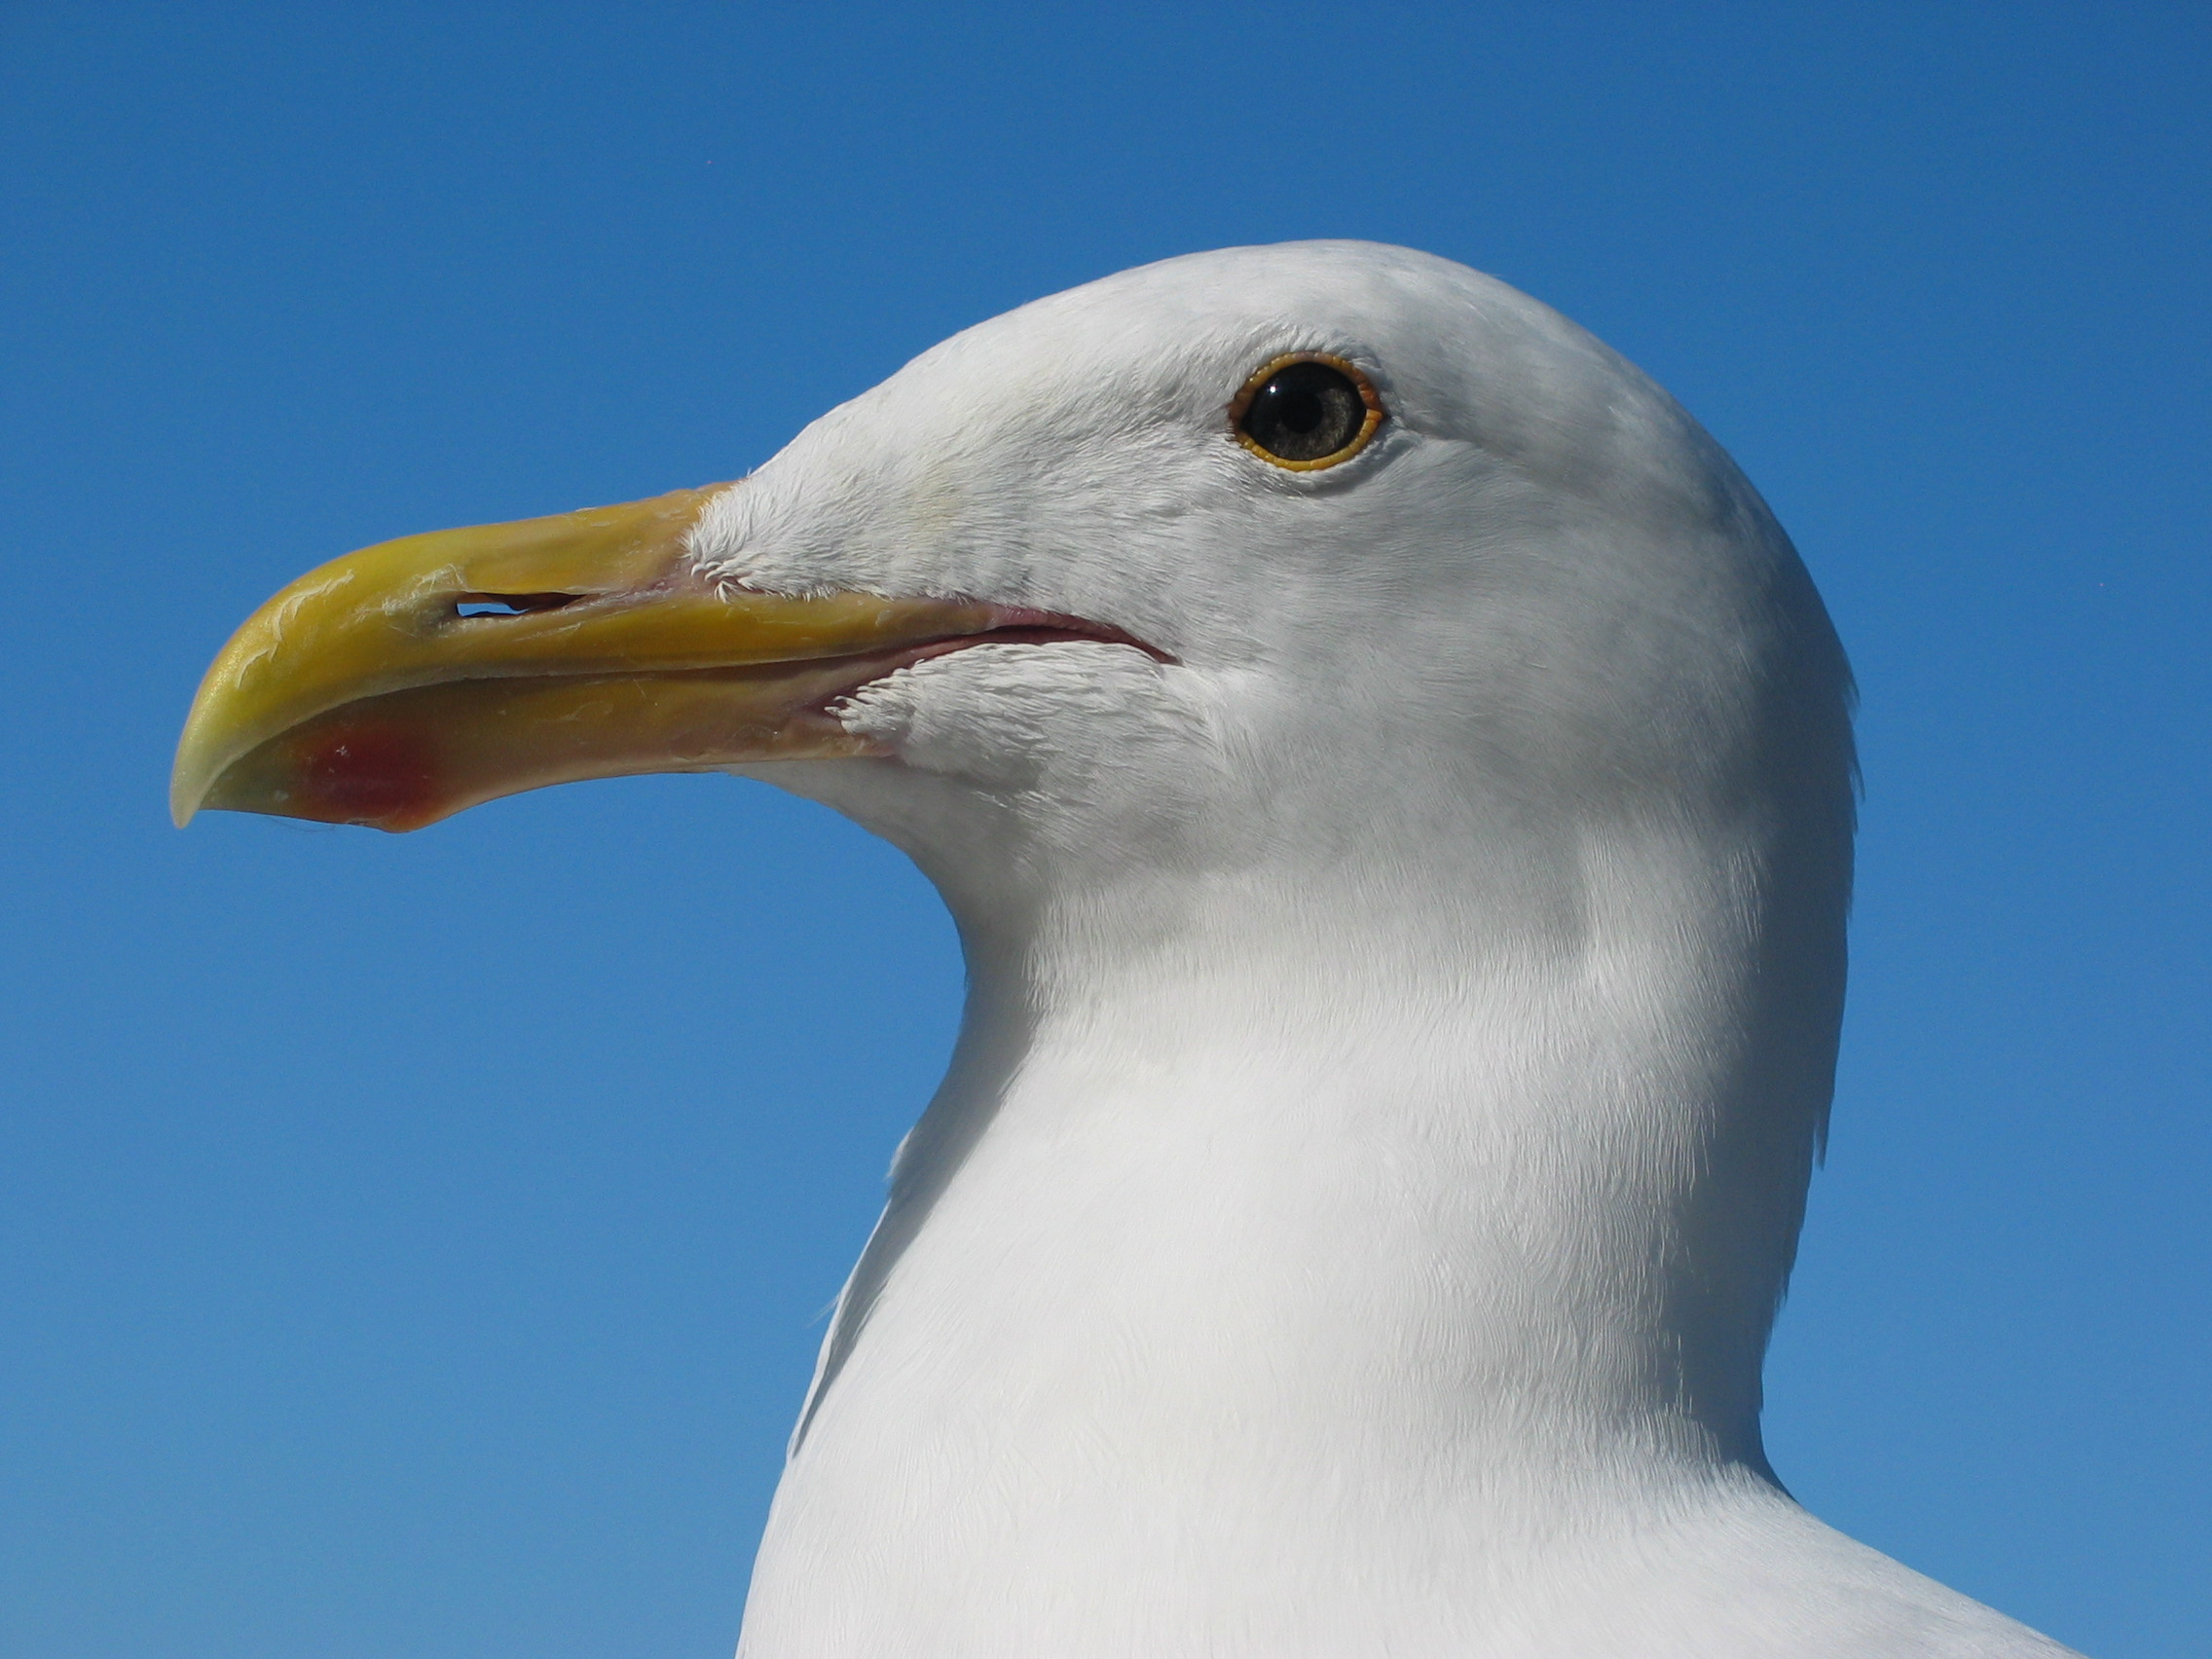
\includegraphics[width=0.8\textwidth]{chapters/images/gull}
  %\caption{A picture of a gull.}
%\end{figure}

\section{3D geometry}

Throughout this work the notion of rigid body transformations and coordinate frames will be used to describe relative motion of bodies.  A rigid body is a solid body where deformation is neglected.  A rigid body transformation is a transformation of some vector space which preserves distances between every pair of points, thus preserving the solid body assumption of rigid bodies. In this work rigid body transformations of 3 dimensional space $\mathbb{R}^3$ will be considered.

A transformation can be described by a rotation followed by a translation.  For $\mathbb{R}^3$ space, there are 3 axes of rotation and 3 axes of translation, and therefore a transformation has 6 degrees of freedom.  These transformations, also known as  'poses', may be described by the special euclidean group $SE(3)$.  Special euclidean groups and Lie Algebra will be covered in \ref{sec:lie_group}.

There are multiple ways to parameterize a rigid body transformation, as different representations for rotations exist.  A common representation is to add a forth homogeneous coordinate and use a 4x4 matrix as follows:
\begin{align}
    \left( 
             \begin{array}{ccc|c}
               &        &   & t_x \\
               & \bv{R} &   & t_y \\
               &        &   & t_z \\ \hline
             0 & 0      & 0 & 1 \end{array} \right) 
\end{align}
R is a 3x3 rotation matrix and $t$ is a 3x1 translation vector.  The forth coordinate can be thought of as the scale, however in this work it will always be set to unity.  This representation means 12 parameters for one rigid body transform, which is very much overparameterization, however this representation allows easier transform composition as when using multiple coordinate systems.

Multiple coordinate systems are used to represent 3D data in different reference frames.  A reference frame is exactly the same as a coordinate system, it can be imagined as being rigidly attached to a solid body.

\begin{figure}[h]
  \centering
      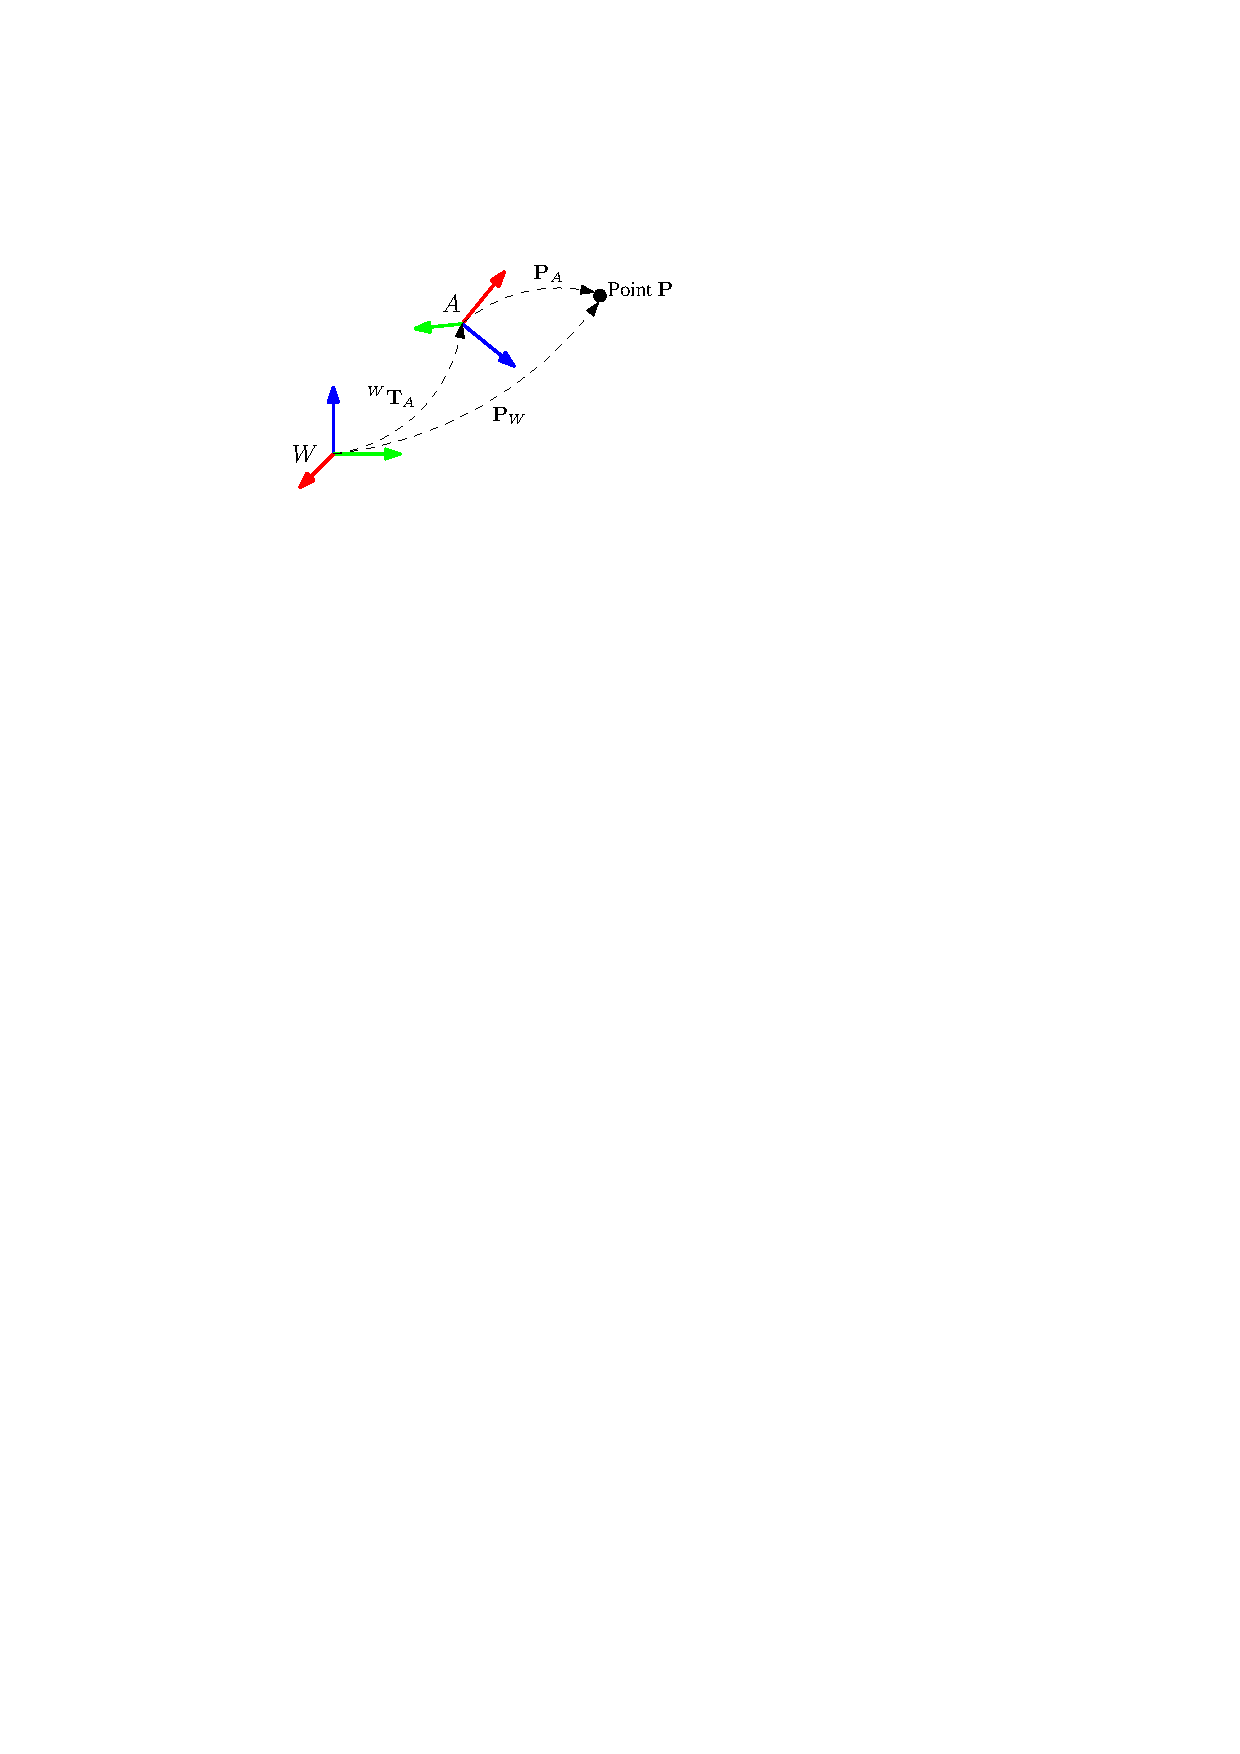
\includegraphics[width=0.5\textwidth]{chapters/images/coord_sys}
  \caption{Coordinate frames. Point $\bv{P}$ may be represented in the coordinate frame  $W$ (fixed world frame) as $\bv{P}_W$ or in the coordinate frame $A$ as $\bv{P}_A$}
  \label{fig:coord_sys}
\end{figure}

\begin{align}
 \bv{P}_W = ^W\bv{T}_A \cdot \bv{P}_A
 \label{eq:a_to_w}
\end{align}

Equation \ref{eq:a_to_w} shows how to transform a point into a different reference frame.  This can be read intuitively as follows; $^W\bv{T}_A$ transforms a point from coordinate frame $A$ being multiplied from the right to coordinate frame $W$.  This same transformation is visualized in Fig. \ref{fig:coord_sys}.  $\bv{T}$ represents a 6 degree of freedom (DoF) rigid body transform, and $\bv{P}$ is a 3 dimensional vector representing a world point. \\
Transformations may be inverted; where 
\begin{align}
 (^W\bv{T}_A)^{-1} = ^A\bv{T}_W
\end{align}
They may also be composed as follows; 
\begin{align}
 ^A\bv{T}_C = ^A\bv{T}_B \cdot ^B\bv{T}_C
\end{align}
Composition is associative but not commutive.  The selected notation helps to disambiguate multiplication order.  As $^A\bv{T}_B$ transforms from frame $B$ to frame $A$, anything being multiplied from the right must be in frame $B$, and anything being multiplied from the left must be in frame $A$.  This notation is consistent throughout the thesis and in the code to avoid confusion.
%TODO: add reference to niko's tutorial

%a point $\bv{P}_A$ multiplied by $^W\bv{T}_A$ from the right transforms it to $\bv{P}_W$.


\section{Lie Groups}
\label{sec:lie_group}

A Lie group $G$ is a set of elements that must satisfy a number of axioms, mainly; the group must be closed under its binary operation, it must be associative, it must have a unique identity element and each element must have a unique inverse.  A Lie group can be thought of as a manifold, allowing calculus on a local space.  The local neighbourhood of any element can be described by its tangent space, which forms the so called Lie Algebra $\mathfrak g$.  For every element there is an exponential map $\exp\colon \mathfrak g \to G$ that maps from Lie algebra to its Lie Group element.  There also exists a logarithmic map $\log\colon G \to \mathfrak g$.  That maps from the Lie Group element to Lie algebra.
%TODO add reference
%link to copy formulas:
%https://www.google.com/url?sa=t&rct=j&q=&esrc=s&source=web&cd=1&cad=rja&ved=0CC4QFjAA&url=http%3A%2F%2Fwww.ai.sri.com%2F~agrawal%2Ficcv05.pdf&ei=tzWQUrW_JYqjrgGgyoHgBQ&usg=AFQjCNEf5gEIFxkeoWnymDixktsxuHRilQ&sig2=94gwoKQvghQEIh_nLeAZ8A&bvm=bv.56988011,d.aWM

In this work, the special euclidean groups $SO(3)$ and $SE(3)$ are used to represent rotations and rigid body transformations respectiveley.  They may be defined as Lie Groups as follows:
 
\begin{align}
  SO(3) = \{ R \mid R \in GL(3), RR^T = I, \det(R) = 1 \} \\
  SE(3) =  \left\{ \left( 
             \begin{array}{cc}
             R & t \\
             0 & 1 \end{array} \right) 
  \in GL(4) \mid R\in SO(3), t \in \mathbb R^3
\right\}
\end{align}
The logarithmic map $SO(3) \to \mathfrak{so}{3}$ is given by
\begin{align}
 \log(R) = \dfrac{\phi}{2\sin(\phi)}(R-R^T) = \hat\omega
\end{align}
Where $\phi$ satisfies
\begin{align}
 Tr(R) = 1 + 2\cos(\phi), |\phi| < \pi
\end{align}
and $\hat\omega$ is the skew symmetric matrix form of the rotation vector $\omega = (\omega_x, \omega_y, \omega_z)$
\begin{align}
 \hat\omega = \left( \begin{array}{ccc}
                      0         & -\omega_z &  \omega_y \\
                      \omega_z  & 0         & -\omega_x \\
                      -\omega_y & \omega_x  & 0
                     \end{array} \right)
\end{align}
The exponential map $\mathfrak{so}(3) \to SO(3)$ is given by
\begin{align}
 \exp(\hat\omega) = I + \dfrac{\sin\|\omega\|}{\|\omega\|}\hat\omega + 
                  \dfrac{1 - \cos\|\omega\|}{\|\omega\|^2}\hat\omega^2
\end{align}
The logarithmic map $SE(3) \to \mathfrak{se}{3}$ is given by
\begin{align}
  \log\left( \begin{array}{cc}
              R & t \\
              0 & 1 
             \end{array} \right)
 =
 \left( \begin{array}{cc}
         \log(R) & A^{-1}t \\
         0 & 0  
        \end{array} \right)
\end{align}
where
\begin{align}
 A^{-1} = I - \dfrac{1}{2}\hat\omega 
          + \dfrac{2\sin\|\omega\| - \|\omega\|(1+\cos\|\omega\|)}
                  {2\|\omega\|^2\sin\|\omega\|}\hat\omega^2
\end{align}
The exponential map $\mathfrak{se}(3) \to SE(3)$ is given by
\begin{align}
 \exp\left(\begin{array}{cc}
             \hat\omega & u \\
             0 & 0  
           \end{array} \right) 
=
  \left(\begin{array}{cc}
          \exp(\hat\omega) & Au \\
          0 & 1 
        \end{array} \right)
\end{align}
where
\begin{align}
 A = I + \dfrac{1 - \cos\|w\|}{\|\omega\|^2}\hat\omega 
          + \dfrac{\|\omega\| - \sin\|\omega\|}
                  {\|\omega\|^3}\hat\omega^2
\end{align}
Note that $\hat\omega$ and $u$ may both be represented by three numbers.  Therefore the exponential map allows a minimal representation of rotation and transformations in terms of parameterization.  This will be utilised later (Sections \ref{sec:oplus}, \ref{sec:error_function}).

\section{Camera Models}
\label{sec:camera_models}
In order to utilise a camera as a sensor, a mapping between image coordinates and world coordinates needs to be derived.  This allows observations of the camera to be transformed into meaningful measurements.  To achieve this mapping a sensor model of the camera is required. This section will cover all the different types of cameras used in this work and corresponding camera models for each. 

\subsection{Pinhole Camera Model}
\label{subsec:pinhole_cam}

%TODO: references

The pinhole camera model is the most basic and common of camera models used in computer vision.  It describes the mathematical relationship between the coordinates of a 3D point in the world and its projection onto an image plane.  This model assumes the aperture of the camera to be an ideal pinhole. It does not consider lenses used to focus light which in reality results in lense distortion.  However practical considerations such as lense distortion can be compensated for.

The pinhole camera model assumes the camera to be a sealed box with a pinhole aperture on one side, and the image plane, or image sensor on the other side.  Having a small aperture blocks most of the light rays from objects in the world and allows a focused and inverted image of the world to be recorded. Fig. \ref{fig:pinhole_inverted}

\begin{figure}[h]
  \centering
    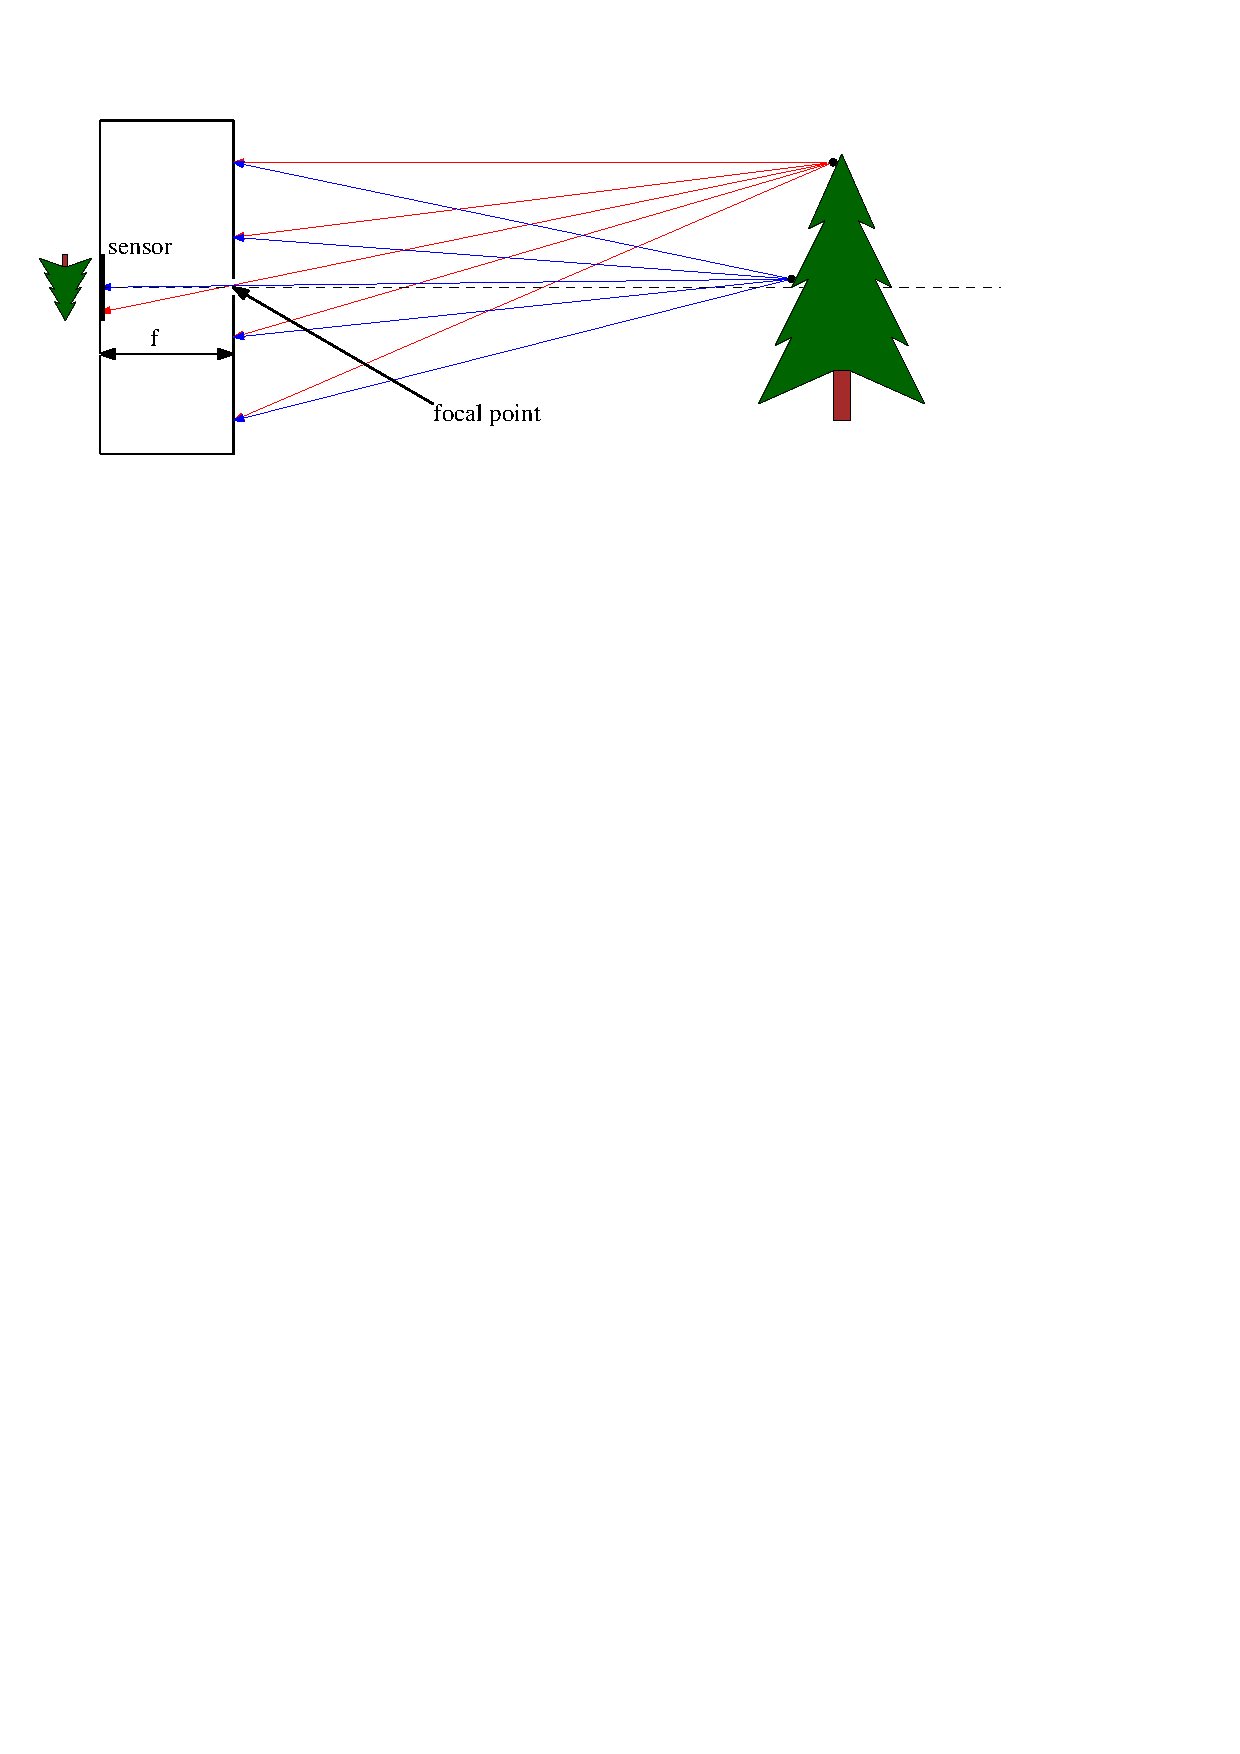
\includegraphics[width=1.0\textwidth]{chapters/images/pinhole_cam_1} \\
  \caption{Pinhole camera model}
  \label{fig:pinhole_inverted}
\end{figure}

\begin{figure}[h]
  \centering
    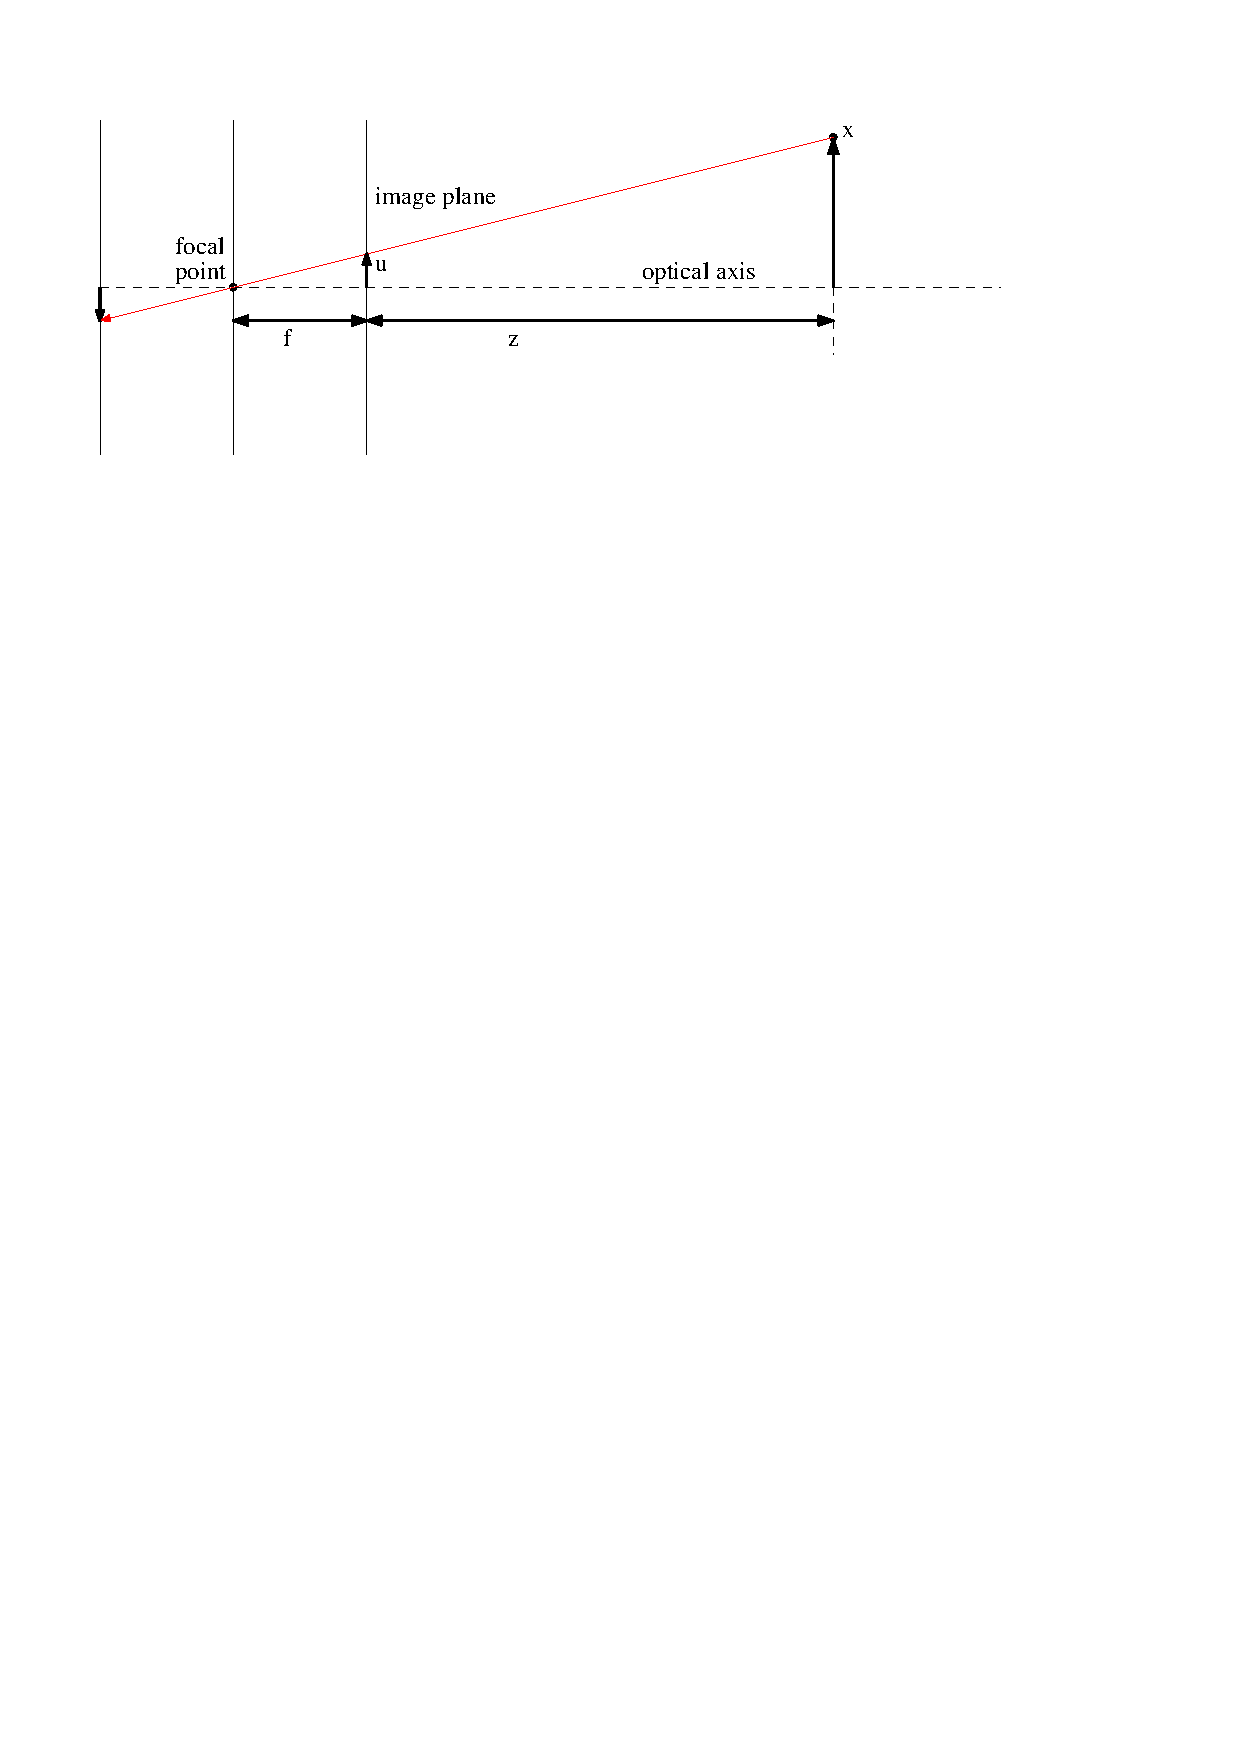
\includegraphics[width=1.0\textwidth]{chapters/images/pinhole_cam_2} \\
  \caption{Pinhole camera model represented with the image plane in front of the focal point}
  \label{fig:pinhole_normal}
\end{figure}

For all intensive purposes, this model can be redrawn as in Fig. \ref{fig:pinhole_normal}. The image plane is inverted and shown reflected in front the of the camera.  In addition it is helpful to express the focal length differently.  Image plane coordinates need to be converted to sensor coordinates (that is, pixel coordinates; u,v).  This can be determined given the image sensor size and its resolution.  As this is linear operation, this conversion may be applied to the metric focal length and thus focal length expressed in pixel units.  Given Fig. \ref{fig:pinhole_normal} and the focal length expressed in pixel units, image coordinates and world coordinates may then be related as follows: 

\begin{align}
  \dfrac{u}{f_x} = \dfrac{x}{z}
\end{align}

This relation is just the x-z plane however the exact same can be applied for the y-z plane.   

Take note that the principle point (center of image) will not be aligned exactly to the center of the image sensor, some offset will exist and will vary from camera to camera.  In addition the focal length varies slightly from camera to camera.  Therefore to properly convert from world coordinates to image coordinates and back both the the x and y focal lengths, and the image coordinates of the principle point need to be determined.  This can be done by performing an intrinsic calibration.
%TODO: references

%http://www.jordicenzano.name/projects/2D-to-3D-Paradigm-overview/camera-model
%use this for picture motivation

\subsection{Lense Distortion}
\label{subsec:lense_distortion}
%TODO: references

The problem with using a pinhole camera in practice is that it does not allow enough light to into the camera, requiring longer exposure time and therefore blurring in the presence of movement. Therefore a double convex lense is often used to focus more light rays onto the sensor and allow a sharper image.  The pinhole camera model may still be used, however now lense distortion needs to be accounted for.  reference shows how to correct for lense distortion given a set of distortion parameters associated with a camera.  These coefficients may be determined through calibration.  Fig. \ref{fig:lense_distortion} shows an example of lense distortion and how it can be compensated for.

Calibration of focal lengths, principle points and distortion coefficients can all be done in one step using a checkerboard of known geometry.  This is called intrinsic calibration.

%When undistorting the image it is not uncommon that parts of the new image around the border will contain no information.  This is overcome by cropping and resizing the image.  This affects calibrated focal length parameters.  However when remapping a new image, new focal lengths can also be determined.

\begin{figure}[h]
  \centering
    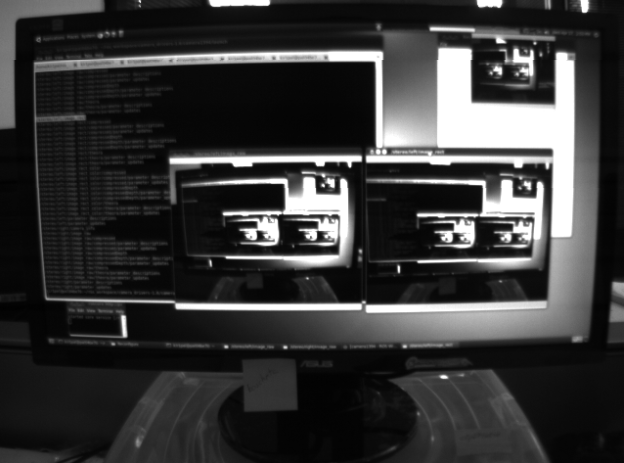
\includegraphics[width=0.49\textwidth]{chapters/images/distorted}
    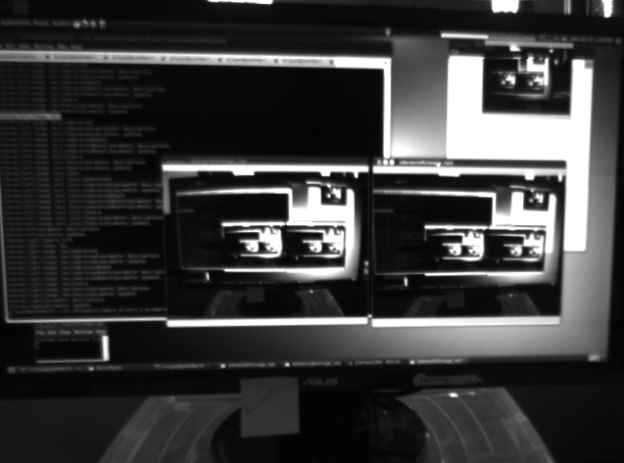
\includegraphics[width=0.49\textwidth]{chapters/images/undistorted}
  \caption{Left: An image with lense distortion.  Right: The same image redrawn with lense distortion considered}
 \label{fig:lense_distortion}
\end{figure}

\subsection{Homogeneous coordinates}

In order to convert from world coordinates to image coordinates and back homogeneous coordinates are used.  This means writing the image coordinates as a $\mathbb R^3$ projective vector $(u, w, 1)^T$.  The conversion from world coordinates to image coordinates may be calculated as follows

\begin{equation}
 \begin{pmatrix}
  u \\
  v \\
  1 
 \end{pmatrix} =
 \begin{pmatrix}
  f_x & 0 & c_x \\
  0 & f_y & c_y \\
  0 & 0   & 1 
 \end{pmatrix}
 \begin{pmatrix}
  X \\ Y \\ Z
 \end{pmatrix}
\end{equation}

Where $f_x$ and $f_y$ are x and y focal lengths and $c_x$ and $c_y$ is the pixel coordinates of the principle point.  The 3x3 matrix is known as the camera matrix, or $\bv K$.

After evaluating the right hand side of the equation, in order to obtain pixel coordinates, the 3D vector needs to be normalised by dividing element wise by the third element:
\begin{equation}
 \begin{pmatrix}
  \frac{X}{Z}  \\
  \frac{Y}{Z}  \\
  \frac{Z}{Z} 
 \end{pmatrix} =
 \begin{pmatrix}
  u \\ v \\ 1
 \end{pmatrix}
\end{equation}

Converting back from image coordinates to world coordinates may be performed by taking the inverse of the camera matrix:

\begin{equation}
 \begin{pmatrix}
  f_x & 0 & c_x \\
  0 & f_y & c_y \\
  0 & 0   & 1 
 \end{pmatrix}^{-1}
 \begin{pmatrix}
  u \\
  v \\
  1 
 \end{pmatrix} =
 \begin{pmatrix}
  X \\ Y \\ Z
 \end{pmatrix}
\end{equation}

This will return a 3D vector that points in the direction of the corresponding 3D coordinates.  Exact 3D coordinates for the point is impossible estimate from a single image as the real world point could lie anywhere on this 3D ray.

\subsection{Stereo Camera}

A stereo camera consists of two regular projective cameras fixed to the same frame with some amount of field of view overlap.  Given that the geometry between the two lenses is known, image points that can be associated between the two images may be triangulated to provide metric, 3D world coordinates with respect to the camera.  A stereo camera can be modelled by two pinhole cameras.  Both cameras can have all their intrinsic parameters calibrated separately as per normal cameras.  

In order to determine 3D data from a stereo camera, first a points need to be associated across both frames.  This means that if there are indiscriminate areas of the stereo image, such as a textureless wall, depth values can not be determined for these pixels. Point association is often achieved via feature matching (Section \ref{subsec:features}).

To make searching for and triangulation of points easier, the two cameras in stereo cameras are often mounted side by side and in the same image plane.  This allows much easier association of points between frames, as a point in one image only needs to be searched for in the other image along the same pixel row.

Having associated points between frames, a disparity value needs to be calculated for each pair.  Disparity is defined as
\begin{align}
  d = u_l - u_r
\end{align}
where $u_l$ is the pixel x coordinate in the left frame and $u_r$ is the pixel x coordinate in right frame.
From Fig. \ref{fig:stereo_disparity}:
\begin{align}
  \dfrac{Z}{b} = \dfrac{f}{d}  \\  
   \Rightarrow Z = \dfrac{f \cdot b}{d}
\end{align}
Where $b$ is the baseline; the distance between the two stereo cameras.
\begin{figure}[h]
  \centering
    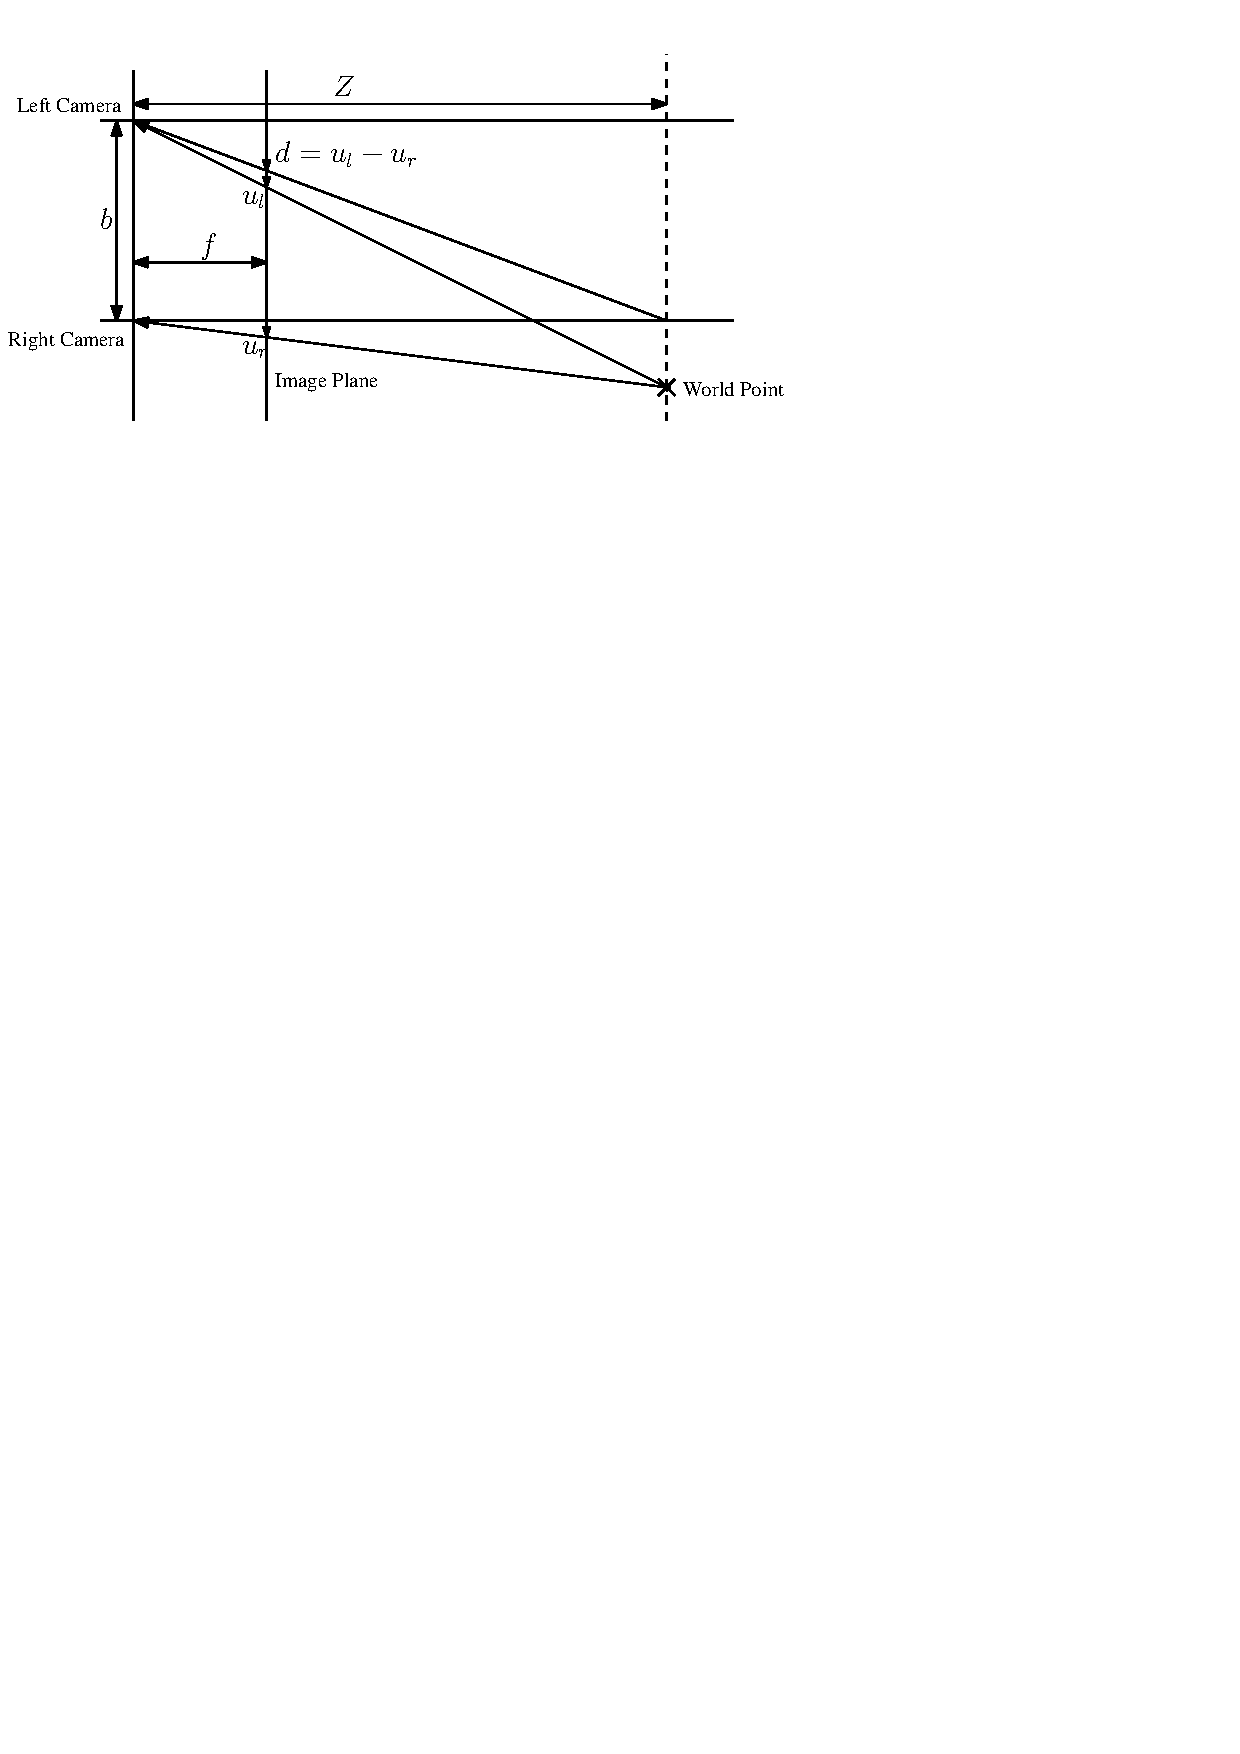
\includegraphics[width=1.0\textwidth]{chapters/images/stereo_disparity}
  \caption{Using disparity to calculate depth.  A fake ray with a image coordinate of $d$ is visualized in the left frame to determine the depth of a world point}
  \label{fig:stereo_disparity}
\end{figure}

Having determined the depth, x and y coordinates may easily be determined using the pinhole camera model.

This is a very straightforward approach to stereo triangulation.  In practice this can be improved by feature point detection with subpixel accuracy, disparity interpolation or dense stereo matching.

%TODO lots and lots of stereo citations

\subsection{Omni-directional Camera}

Some stuff

\begin{figure}[h]
  \centering
    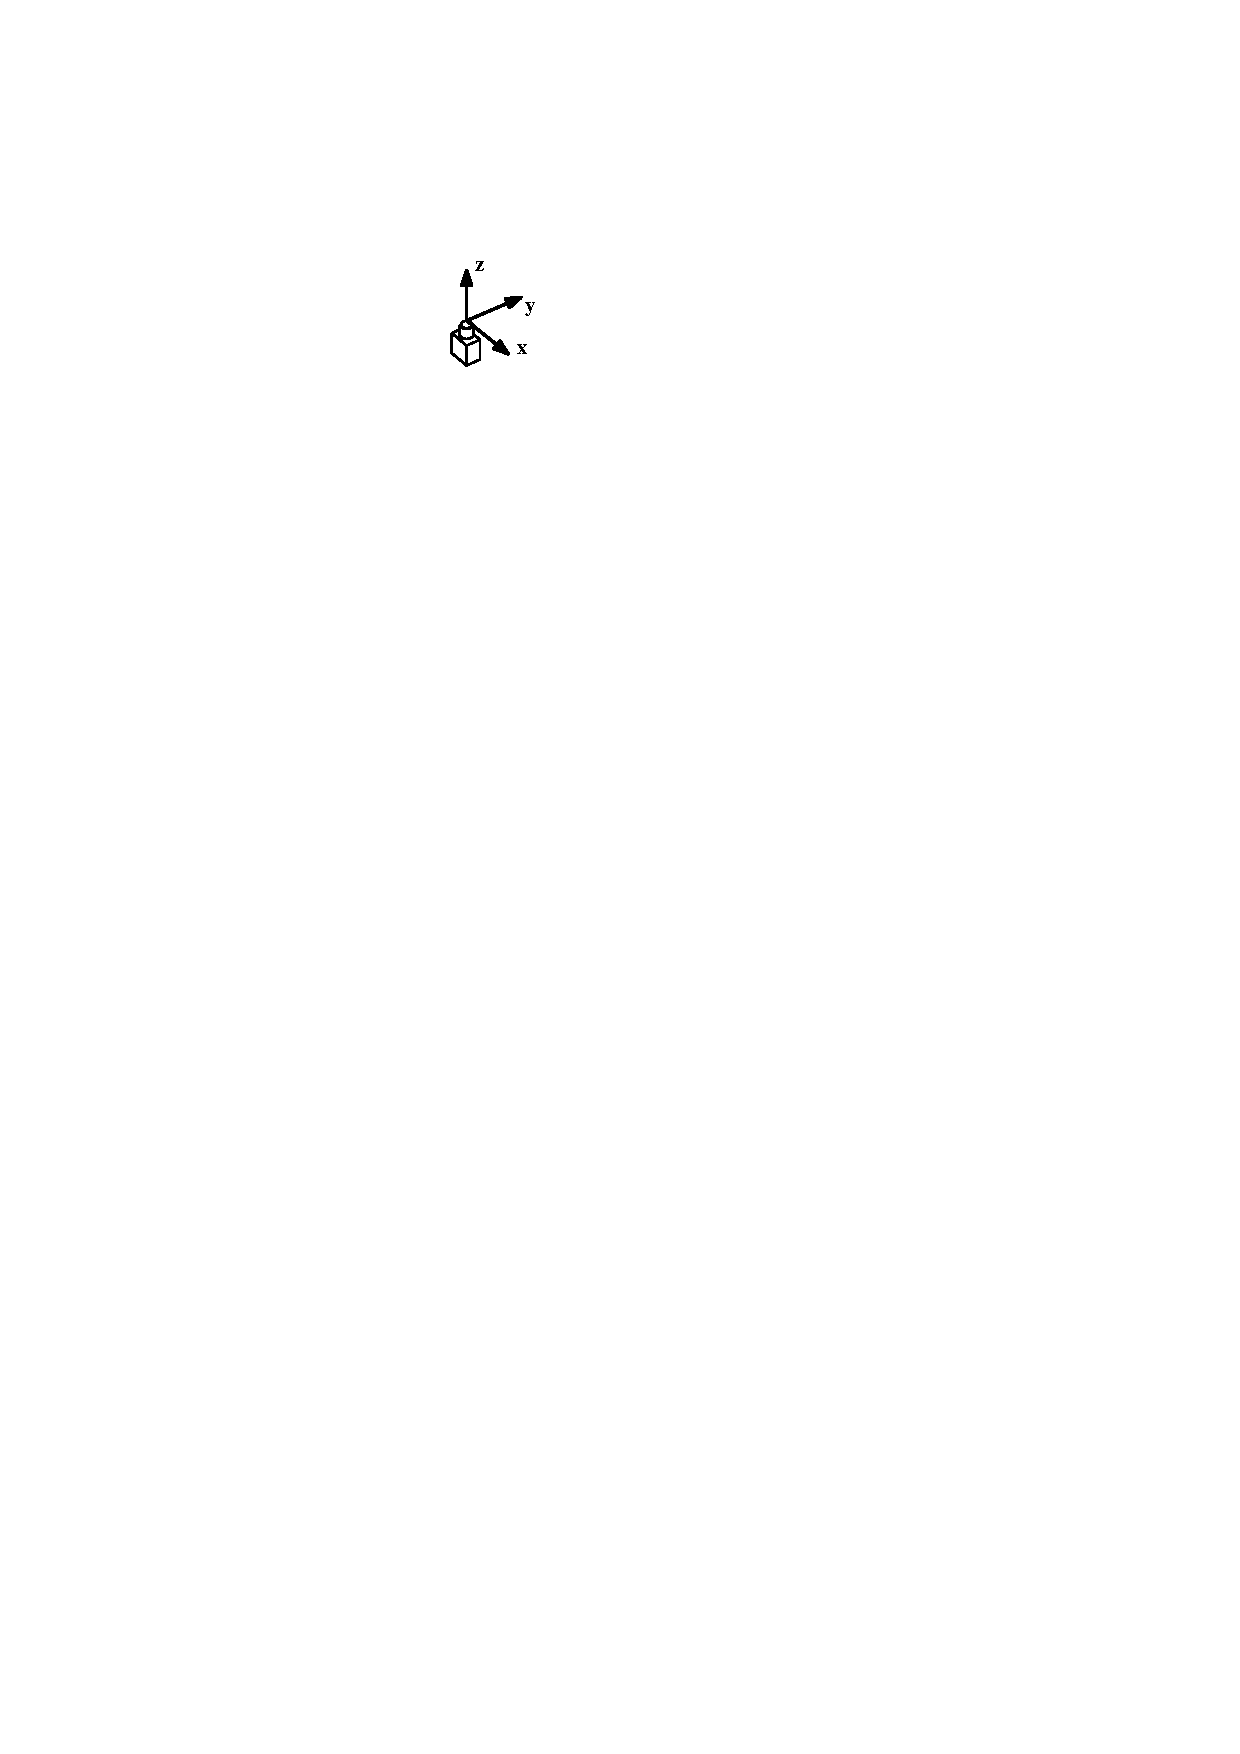
\includegraphics[width=0.15\textwidth]{chapters/images/omni_coord_sys}
  \caption{Omni camera coordinate frame}
  \label{fig:omni_coord_sys}
\end{figure}
% ask matthias for literature

\section{Computer Vision Basics}
\label{sec:computer_vision}

\subsection{Feature point detection and extraction}
\label{subsec:features}

Outline what is feature point detection, description and matching, why we need it.  Mention SIFT and SURF and cite them.  Mention that we used a GPU implemtation of SIFT, cite the ETH paper. Mention a bunch of other descriptors, cite them as well.

\subsection{Feature Matching}

include circular matching

\subsection{Reprojection Error}

Reprojection error is an important concept that will be referred to many times in this work.  It is a very powerful tool to more accurately model the cameras accuracy as a sensor.
%TODO

\subsection{RANSAC}
\label{subsec:RANSAC}

explain this cos its easy and fun.  Cite a paper

\subsection{Geometry estimation}

\subsubsection{5 point algorithm}
\label{subsec:5point}
%ask for matthias for relavent literature

\subsubsection{p3p algorithm}
\label{subsec:p3p}
%ask for matthias for relavent literature

\subsubsection{Point triangulation}
\label{subsec:point_triangulation}

%ask for matthias for relavent literature

\subsubsection{Stereo pose estimation}
\label{subsec:horn}

Umeyama (PCL) \newline 
Horn (UVM) \newline

\section{Place Recognition}
\label{sec:bag_of_words}
Bag of words \\
Vocabulary tree, Nister \\
fabmap

\section{SLAM}
\label{sec:slam}

Simulataneous Localization and Mapping (SLAM) is the technique of building a map of a previously
unexplored area whilst simultaneously determining a position (localizing) within that map.  The
traditional approach for SLAM can be split into 4 steps.
\begin{enumerate} \itemsep1pt \parskip0pt \parsep0pt
 \item Feature extraction
 \item Data association
 \item Pose estimation
 \item Global Optimization
\end{enumerate}

%TODO: cite kalman filter
Feature extraction involves finding unique features within the sensor data that can be later reidentified in future sensor readings.  These features denote individual observations of a landmark through the eyes of a sensor.  A landmark can be thought of as a real world object which can be observed by a sensor.  Data association is the process of matching multiple observations of a single landmark over multiple sensor readings, in essence tracking the landmarks.  Take for example a robot doing 2D indoor SLAM with a 2D laser scanner.  A simple feature would be corners detected in the laser data.  These are observations of real world corners between walls, or any object within range of the laser scanner that would cause a sharp angle to be observed.  These real corners or objects can be thought of as landmarks.

\begin{figure}[h]
  \centering
    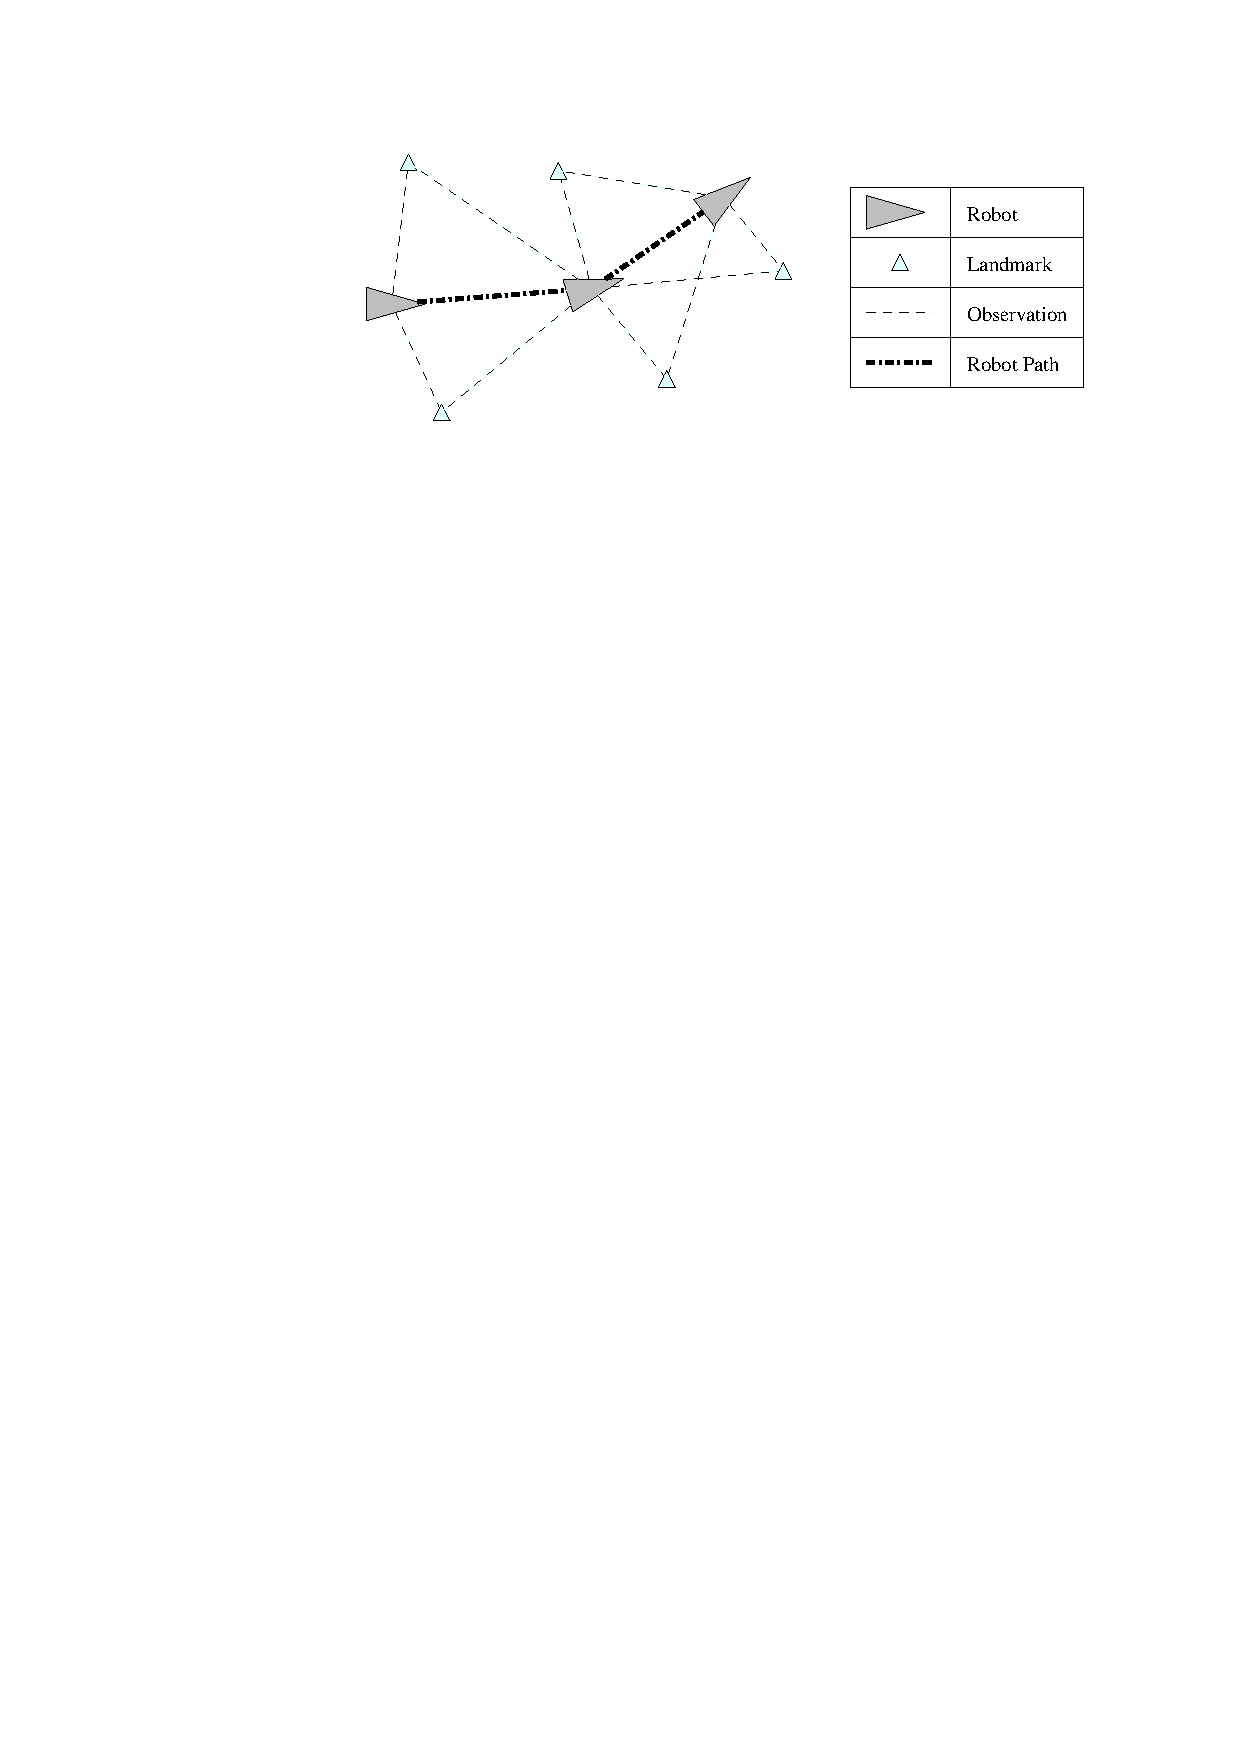
\includegraphics[width=0.8\textwidth]{chapters/images/2D_SLAM}
  \caption{Simple generic SLAM representation }
\end{figure}

Pose estimation involves using the information of how multiple landmarks have moved over time with respect to the robot/sensor, in order to determine how the robot has moved with respect to those landmarks.  

At this stage it is possible to calculate a map and trajectory by performing pose estimation between the current and previous frame and chaining all consecutive pose estimations together.  However this is a rather simple approach, as no temporal information (i.e. information from older sensors data or older poses) is considered when determining the current pose.  Therefore it is desirable to have some 'global optimization' strategy to optimize the trajectory and map over non consecutive sensor data.

There are two established approaches to address this.  The first and more well known approach is the use of filtering, e.g. the Extended Kalman Filter (EKF) or the Particle Filter.  In the case of Kalman filtering, landmark positions are added to the system state.  In the case of particle filtering, many initial random robot poses are considered and the particles converge to a solution.
%TODO: EKF, particle, davidson

In more recent times graph optimization approaches have become popular as not only do they scale better to larger maps, but they retain original measurements of the world rather than fusing them with the robot state at the time of observation as per filtering.  This has been proved to improve accuracy of SLAM systems.
%TODO: hauke why filter

\section{Visual SLAM}

SLAM has taken many forms depending on sensors available. Visual SLAM (VSLAM) denotes performing SLAM using some kind of camera.  In recent times, a plethora of VSLAM algorithms for monocular cameras (cite andrew davidson slam, ptam, something else), stereo cameras (more citations) and RGBD cameras (rgbdslam, kinfu, kintinuous) have been developed.

\subsection{Basic VSLAM pipeline}

The following is a description of a basic pipeline for VSLAM.  Whilst the SLAM system utilised by this work as an underlying framework is somewhat more complex, this section shows how all the algorithms in Sections \ref{sec:camera_models}, \ref{sec:computer_vision}, and \ref{sec:bag_of_words} may be used together to form a complete SLAM pipeline.  The SLAM system actually used will be discussed in more detail in Section \ref{chapter:ScaViSLAM}

The feature extraction in VSLAM involves using image feature detectors/descriptors (\ref{subsec:features}).  A feature point may then be considered as a single observation of a landmark.  This observation may be represented as a 3D ray from the current camera pose to the landmark by making use of the camera model (\ref{subsec:pinhole_cam}).  Multiple observations over multiple frames allow for multiple rays to intersect at this landmark, and therefore a 3D position of the landmark may be estimated using triangulation (\ref{subsec:point_triangulation}). In the case of a stereo camera, the 3D estimate more or less comes for free, as landmarks may be triangulated from left and right camera frame.

The data association stage is performed by excectuting feature matching across different camera frames. Pose estimation is commonly achieved by utilising the RANSAC algorithm (\ref{subsec:RANSAC}) This can be coupled with the 5 point algorithm (\ref{subsec:5point}) in the case of initializing monocular SLAM (2D-2D correspondances), the p3p algorithm (\ref{subsec:p3p}) for tracking in monocular SLAM (2D-3D correspondances), or with Umeyama/Horn (\ref{subsec:horn}) for stereo or RGBD, (3D-3D correspondances). The model in this case is the 6 DoF transformation between frames. 

The error may be either euclidean distance between points or reprojection error after the all points have been transformed to one of the frames for comparison by applying the transformation. Eq. \ref{eq:ransac_error} provides an example using euclidean distance as an error function for points with estimated 3D locations.

\begin{figure}[h]
 \centering
 \begin{math}
  \bv{e} = \sum\limits_{i=0}^n \| (\bv p_A)_i - ^A\bv T_B \cdot (\bv p_B)_i \|
 \end{math}
 \caption{RANSAC error function example using euclidean distance}
 \label{eq:ransac_error}
\end{figure}

Global optimization may be done with filtering.  Davidson et al. has a prominent example of such a system.  However as mentioned before graph optimzation has been shown to be more accurate and is now more common in VSLAM.  The formulation of graph optimization will be expanded on in Section \ref{subsec:graph_slam}.
%TODO davidson, ptam

\subsection{Keyframe SLAM}

As mentioned in Section \ref{sec:slam}, graph optimization allows all measurements such as pose estimations, feature keypoint locations or landmark positions to be stored and all combined in one global optimization step.  However if every camera frame were to be considered, with an average video camera operating at 30Hz, this would quickly lead to a computationally intractable problem.  Therefore some strategy is required to reduce the amount of data to be optimized.

Keyframe SLAM provides such a strategy.  The idea of keyframe SLAM is that certain camera frames are choosen as 'keyframes'.  Keyframes along with triangulated landmarks are added to the graph to be optimized.  For all other frames inbetween keyframes, tracking is still performed to provide an accurate current pose, however any information gathered does not contribute to the global map.  An illustration of keyframe SLAM can be seen in Fig. \ref{fig:keyframe_slam}.  Using this strategy, the graph optimization performs a bundle adjustment over all keyframe poses and landmark positions, based on shared observations of landmarks. 

\begin{figure}[h]
  \centering
    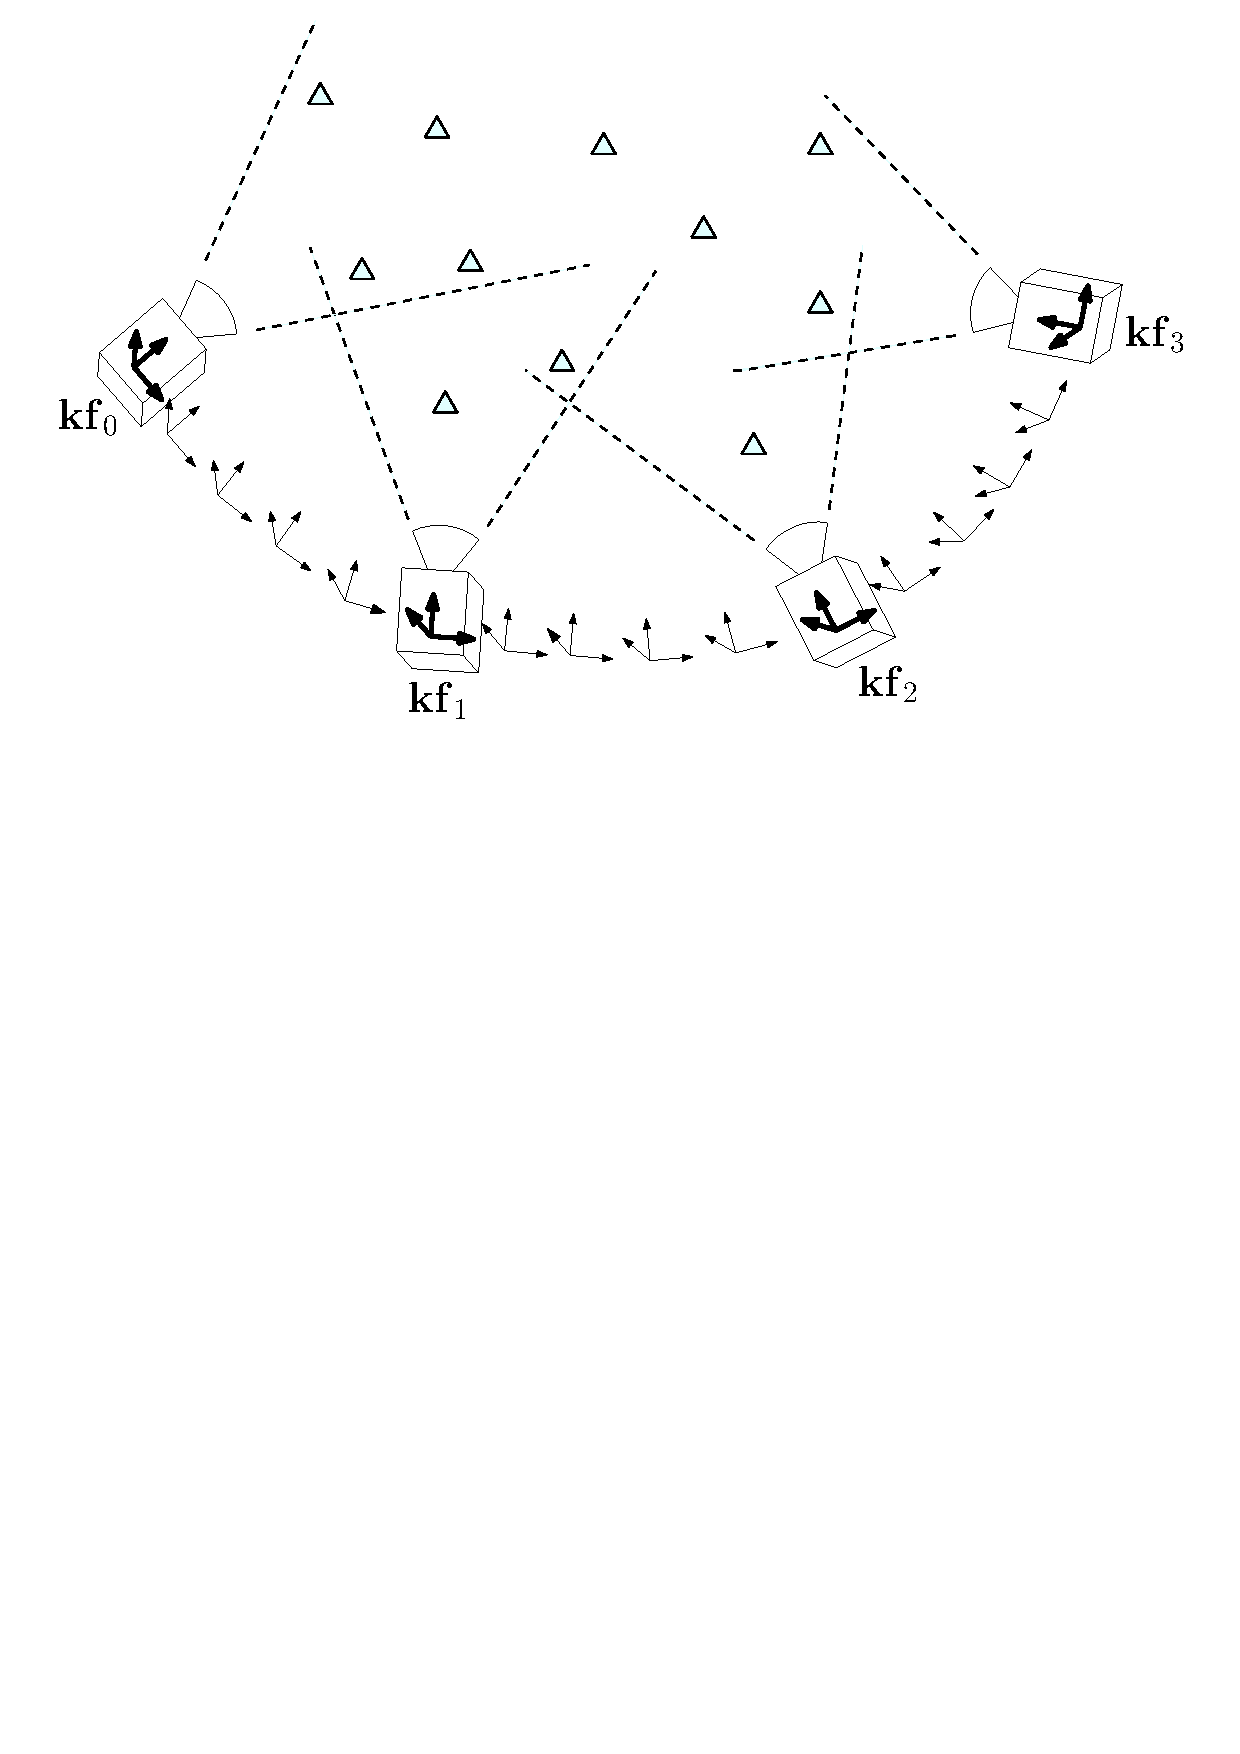
\includegraphics[width=0.7\textwidth]{chapters/images/keyframes}
  \caption{Keyframe SLAM.  The coordinate systems with cameras overlayed represent keyframes whilst the other ones represent intermediate frames}
  \label{fig:keyframe_slam}
\end{figure}

Keyframes may be selected based on a set of criteria such as minimum number of landmarks still visible from the previous keyframe, distance traveled from the previous keyframe, absolute value of rotation to the previous keyframe or time elapsed since the last keyframe was created. 

The structure of keyframe SLAM lends itself to separate the mapping and tracking pipelines to different threads.  PTAM is a noteable example of which.  In this case the tracking thread is optimized to excectute quickly, so it can run in realtime without skipping frames, and the mapping thread is responsible for graph optimization and may run slower.  This allows for an accurate estimation and fast update rate, and also a globally consistent map.
%TODO: cite PTAM

%The main idea behind keyframe SLAM is to divide the tasks of localization and mapping, and have them run in parallel is separate threads.  The mapping thread defines a keyframe to track against. This amounts to a global pose of the keyframe, as well as a number of landmarks visible from that keyframe recorded relative to that keyframe pose.  The localization thread localizes the camera with respect to that keyframe.  If the camera moves or rotates a significant distance away from the active keyframe, a new keyframe will be created with a known transformation to the previous keyframe.

%The intent is to have a fast localization thread that runs in realtime providing an accurate pose estimation with respect to the keyframe.  The mapping thread that deals with the keyframe runs at a much lower framerate, and handles changing the keyframe, global optimization(?), something else. The overall outcome is a system that provides an accurate pose in global coordinates with a fast update rate, as well as a globally consistent map.

\subsection{Loop Closure}
\label{subsec:loop_closure}

A common problem with visual SLAM systems is that the pose estimation between frames is not perfectly accurate.  While locally this is not a problem, if the camera is to move a long distance this error will accumulate, as the current pose is the product of all previous poses chained together.  This effect can easily be demonstrated by performing a long trajectory and returning to the start point.  Whilst the camera is in its original position, the estimated pose will be some offset from the origin. See Fig. \ref{fig:loop_closure}.

\begin{figure}[h]
  \centering
    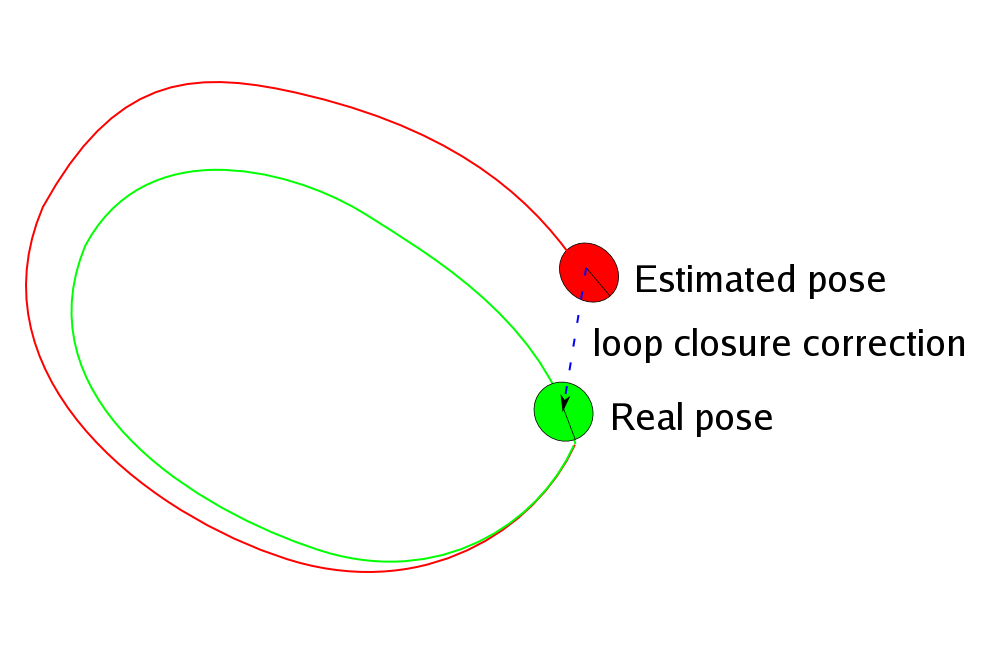
\includegraphics[width=0.5\textwidth]{chapters/images/loop-closure}
  \caption{Loop Closure}
  \label{fig:loop_closure}
\end{figure}
%TODO: change this with a before after shots from presentation g2o graph

It is possible to compensate for this drift by performing 'large loop closures'. After returning to a previous location, the current frame can be registered against an earlier recorded frame at this same location using the standard pipeline of pose estimation based on shared landmark observations.  The current pose is then corrected to the correct position by adjusting all of the previous poses slightly.  This adjustment may be performed efficiently and optimally using graph optimization.

\section{Graph Optimization}
\label{subsec:graph_slam}

To express an optimization problem as a graph, one can think of vertices as being variables, or states, to optimize over, and edges as being constraints for 1 or more vertices.  Edges for a single vertex are called unary edges, for two vertices binary edges and more than 2 multi edges.  Vertex states may be one or more dimensions.  Having said that, vertices may also be used as parameters in the optimization problem.  Error functions to minimise are then defined as how well vertex states fit their edge constraints.  Due to the fact an edge may connect more than two vertices, this type of graph is referred to as a hyper-graph.

An example of how a simple SLAM problem may be expressed as a hyper-graph is shown below.
\begin{figure}[h]
  \centering
      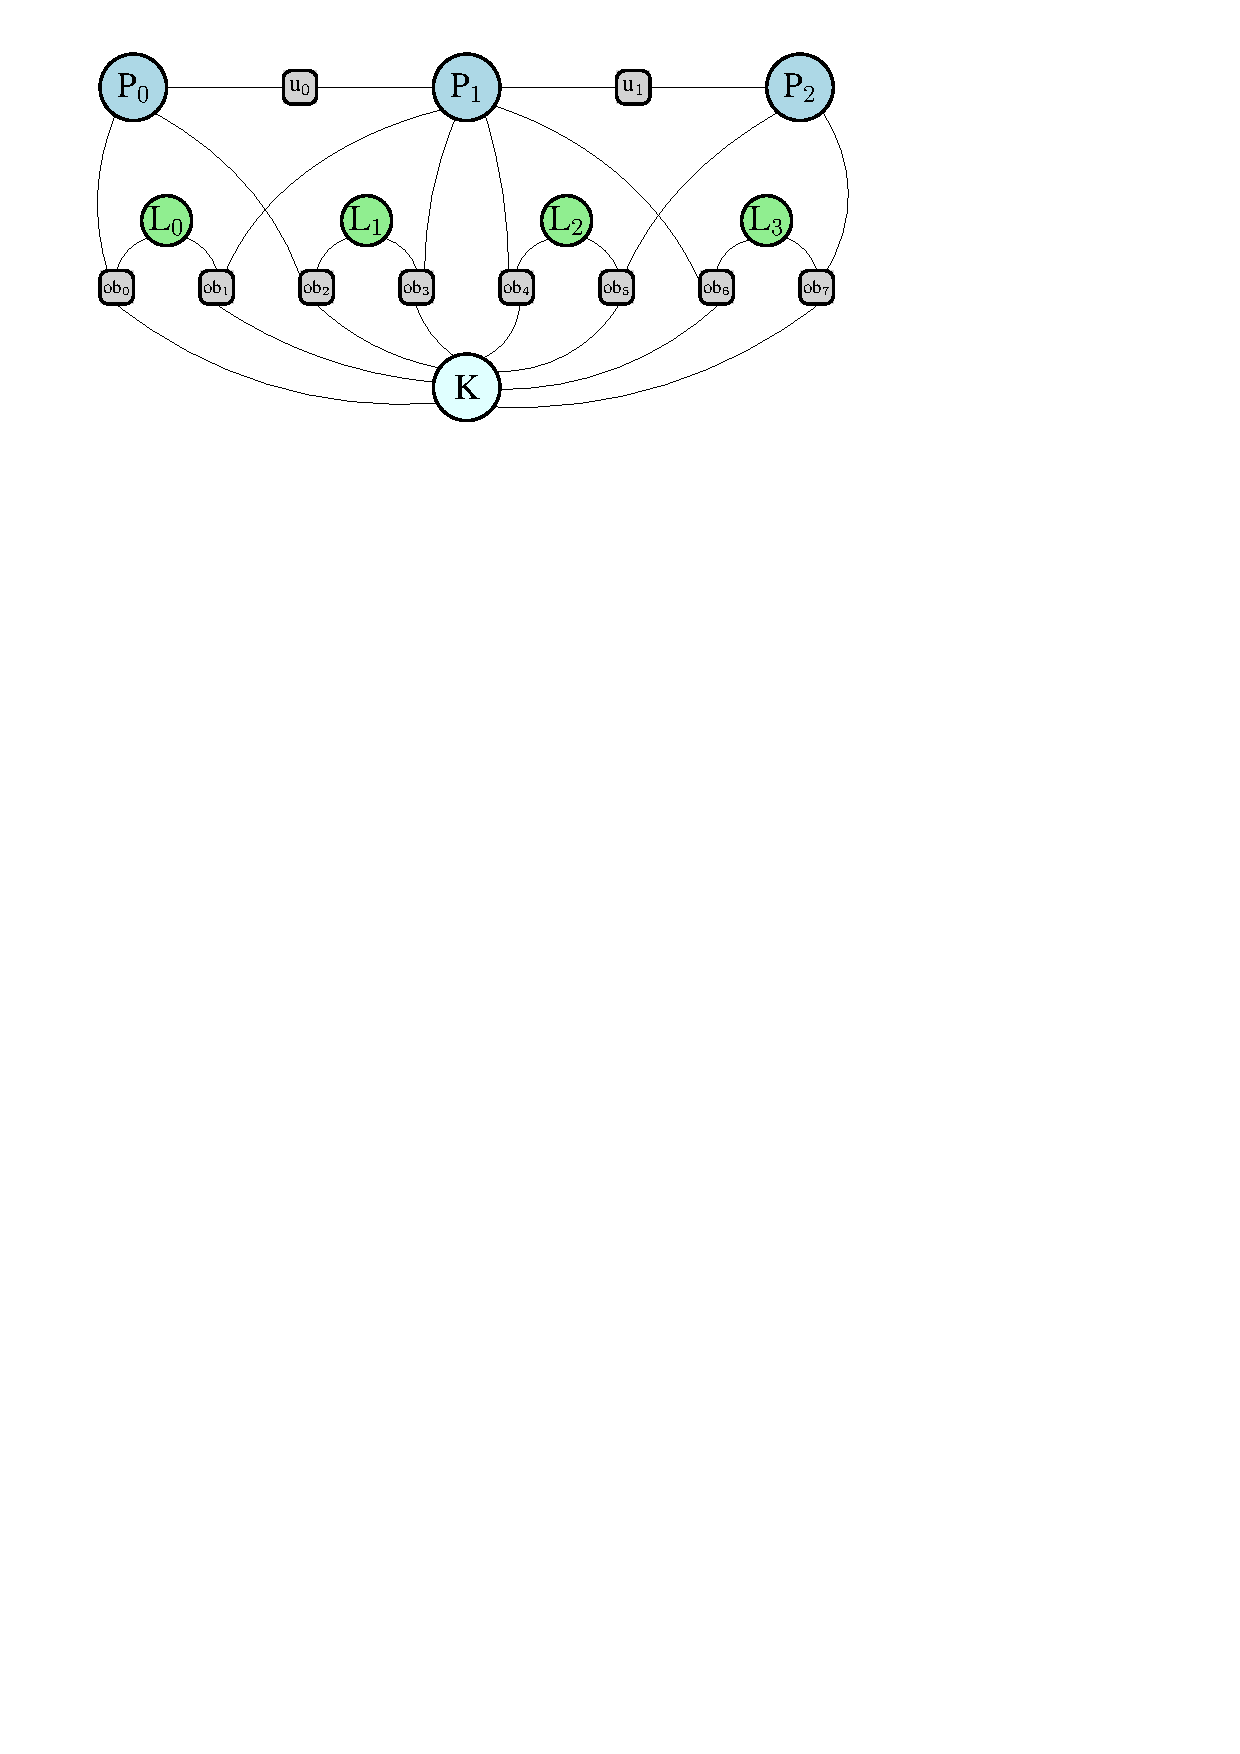
\includegraphics[width=0.8\textwidth]{chapters/images/simple_graph}
  \caption{A simple SLAM graph for a generic robot.  Circles are vertices to optimize over, and
squares are edges, which in this case are measurements}
\end{figure}

The diagram shows robot poses as $\bv P_i$.  These poses could be represented by any number of dimensions. In the case of an exploratory robot, this is likely to be 3 dimensional (x, y, and yaw for movement on a fixed plane), or 6 dimensional (x, y, z, rotation about x, rotation about y, rotation about z).  $\bv U_i$ are binary edges, representing odometry measurements between robot poses. These are measurements or constraints and will remain unchanged during optimization.  
$\bv L_i$ represents unique landmarks that the robot can sense and make some form of measurement relative to its own position, as well as re-identify in different robot poses.  A landmark could be a corner from a laser scan or a feature point in a camera image.  $\bv K$ represents calibration parameters of the sensor.  This could be something like an offset, camera intrinsic parameters, or an extrinsic parameter to transform the sensor readings from the sensor frame to the robot frame.  $\bv {ob}_i$ are observation multi-edges, between a robot pose, a landmark, and the calibration parameter.

Such an example of graph optimization would allow an optimization of the poses of the robot, positions of the landmarks, and the sensor calibration, based on all odometry and observation measurements.

In order to compute this optimization, the generic graph problem may be represented mathematically as follows:

 \begin{align}
   \bv{F}(\bv x) &= \sum\limits_{K \in C}^{} 
                 \bv e_k(\bv x_k, \bv z_k)^T 
                 \bv \Omega_k
                 \bv e_k(\bv x_k, \bv z_k)  \\ 
   \bv x^* &= \operatornamewithlimits{argmin}\limits_{\bv x}\bv{F}(\bv x)
 \end{align}

\begin{itemize}
 \item $\bv x$ is a vector of parameter sets, whereby each $\bv x_i$ is a parameter block
 \item $\bv x_k$ is a set of parameters involved in the $k$th constraint
 \item $\bv z_k$ is a constraint or measurement relating to parameter $\bv x_k$
 \item $\bv \Omega_k$ is the information matrix for $\bv z_k$.  This can be used to weight this constraint
 \item $\bv e_k(\bv x_k, \bv z_k)$ is the error function that measures how well parameter block $\bv x_k$ satisfies $\bv z_k$.  If for instance $\bv z_k$ directly measured $\bv x_k$, then a straightforward error function would be $\bv e_k(\bv x_k, \bv z_k) = \bv x_k - \bv z_k $
\end{itemize}

\subsection{Solving the least squares problem}

%TODO: citations
A numerical solution to eq. 4.2 can be performed using a non linear solver such as Gauss-Newton or Levenberg-Marquardt (cite, cite).  The error function can be approximated by its first order Taylor expansion around the current initial guess $\breve{\bv x}$

\begin{align}
  \bv e_k(\breve{\bv x}_k + \Delta \bv x_k) &= \bv e_k(\breve{\bv x} + \Delta \bv x) \\
      & \simeq \bv e_k + \bv J_k \Delta \bv x
\end{align}

$\bv J_k$ is the Jacobian of $\bv e_k(\bv x)$ computed in $\breve{\bv x}$.  Substituting eq(4.4) as the error function in eq(4.1), one obtains:

\begin{align}
  \bv F(\breve{\bv x} + \Delta \bv x) &= \bv e_k(\breve{\bv x} + \Delta \bv x)^T \bv \Omega_k \bv e_k(\breve{\bv x} + \Delta \bv x) \\
  & \simeq (\bv e_k + \bv J_k \Delta \bv x)^T 
    \bv \Omega_k 
    (\bv e_k + \bv J_k \Delta \bv x) \\
  &= \bv e_k^T \bv \Omega_k \bv e_k 
    + 2 \bv e_k^T \bv \Omega_k \bv J_k \Delta \bv x 
    + \Delta \bv x^T \bv J_k^T \bv \Omega_k \bv J_k \Delta \bv x \\
  &= c_k + 2\bv b_k \Delta \bv x + \Delta \bv x \bv H_k \Delta \bv x
\end{align}

Where $c_k = \bv e_k^T \bv \Omega_k \bv e_k$, $\bv b_k = \bv e_k^T \bv \Omega_k \bv J_k$ and $\bv H_k = \bv J_k^T \bv \Omega_k \bv J_k$. This quadratic form can then be minimized in $\Delta \bv x$ by solving the linear system

\begin{align}
   \bv H \Delta \bv x^* = -\bv b
\end{align}

$\bv H$ is a very large sparse square matrix.  It is mostly zeros; it only contains non zero values where there is a constraint connecting blocks.  This matrix can be efficiently solved by taking advantage of the fact that it is sparse, for instance, by sparse Cholesky factorization.
%TODO cite cholmod csparse

\subsection{Update Operator}
\label{sec:oplus}

As part of the SLAM problem, it is common to have parameterization in non Euclidean space.  For instance, a 3 dimensional pose $SE(3)$ is described by a translational part $\mathbb{R}^3$, which is clearly Euclidean, and a rotational component $SO(3)$ which is not euclidean.  The rotation part is often described in some over parameterized way, for instance quaternions or rotational matrices.  

The solver is mostly likely to be agnostic about the exact representation of the vertex state, it just knows the degrees of freedom of a vertex.  This means during optimization the optimizer will provide increments to the vertex in the form of a vector with as many values as degrees of freedom.  If the rotational part was expressed as a rotation matrix, then somehow this 3D vector needs to be applied to the matrix in a sensible way.  The vector may not be simply added or multiplied to the matrix due to the non euclidean nature of this representation.

One way to deal with this is to optimize over all degrees of freedom of the over parameterized representation, in this case 9 degrees for an $SO(3)$ + 3 for the translation part, therefore 12 degrees per vertex, however this makes the problem more complex and can introduce error.  Another way is to use the 3D increment vector as Euler angles, however singularities could occur due to Gimbal lock.

A better idea is to consider the problem space as a manifold.  A manifold is a space that globally may not be euclidean, although locally can be considered euclidean.  Then one needs to define an operator, denoted $\boxplus$, which maps a local variation $\Delta\bv x$ in Euclidean space on to the Manifold. $\bv e_k(\bv x_k \boxplus \Delta\bv x$)

The Lie algebra provides a compact representation of the element, and therefore we can use the exponential map $\exp\colon \mathfrak g \to G$ for the $\boxplus$ operator.  For a further explanation of Lie groups and the logarithmic map, please see \ref{sec:lie_group}

\subsection{Error functions}
\label{sec:error_function}
The error function $\bv e_k(\bv x_k, \bv z_k)$ measures how well the vertices fit the the edge that they are connected to.  A similar problem is encountered as for vertex increments when calculating error for the case of non euclidean parameterization.  Again for the example of the $SE(3)$ pose, in this case the error, which could be described as an $SE(3)$ pose, needs to be converted to some minimal vector form for the optimizer.  In this case the  logarithmic mapping $\log\colon G \to \mathfrak g$ can be used to achieve this conversion. More details see \ref{sec:lie_group}

%\subsubsection{Robust least squares}
%TODO huber fill in
%Use huber instead of squares to make robust against outliers. !
%CBF

\section{Related work}

google some stuff!